\cohead{\Large\textbf{Steigungswinkel}}
\fakesubsection{Steigungswinkel}
\begin{minipage}[t]{\textwidth}
	\centering
	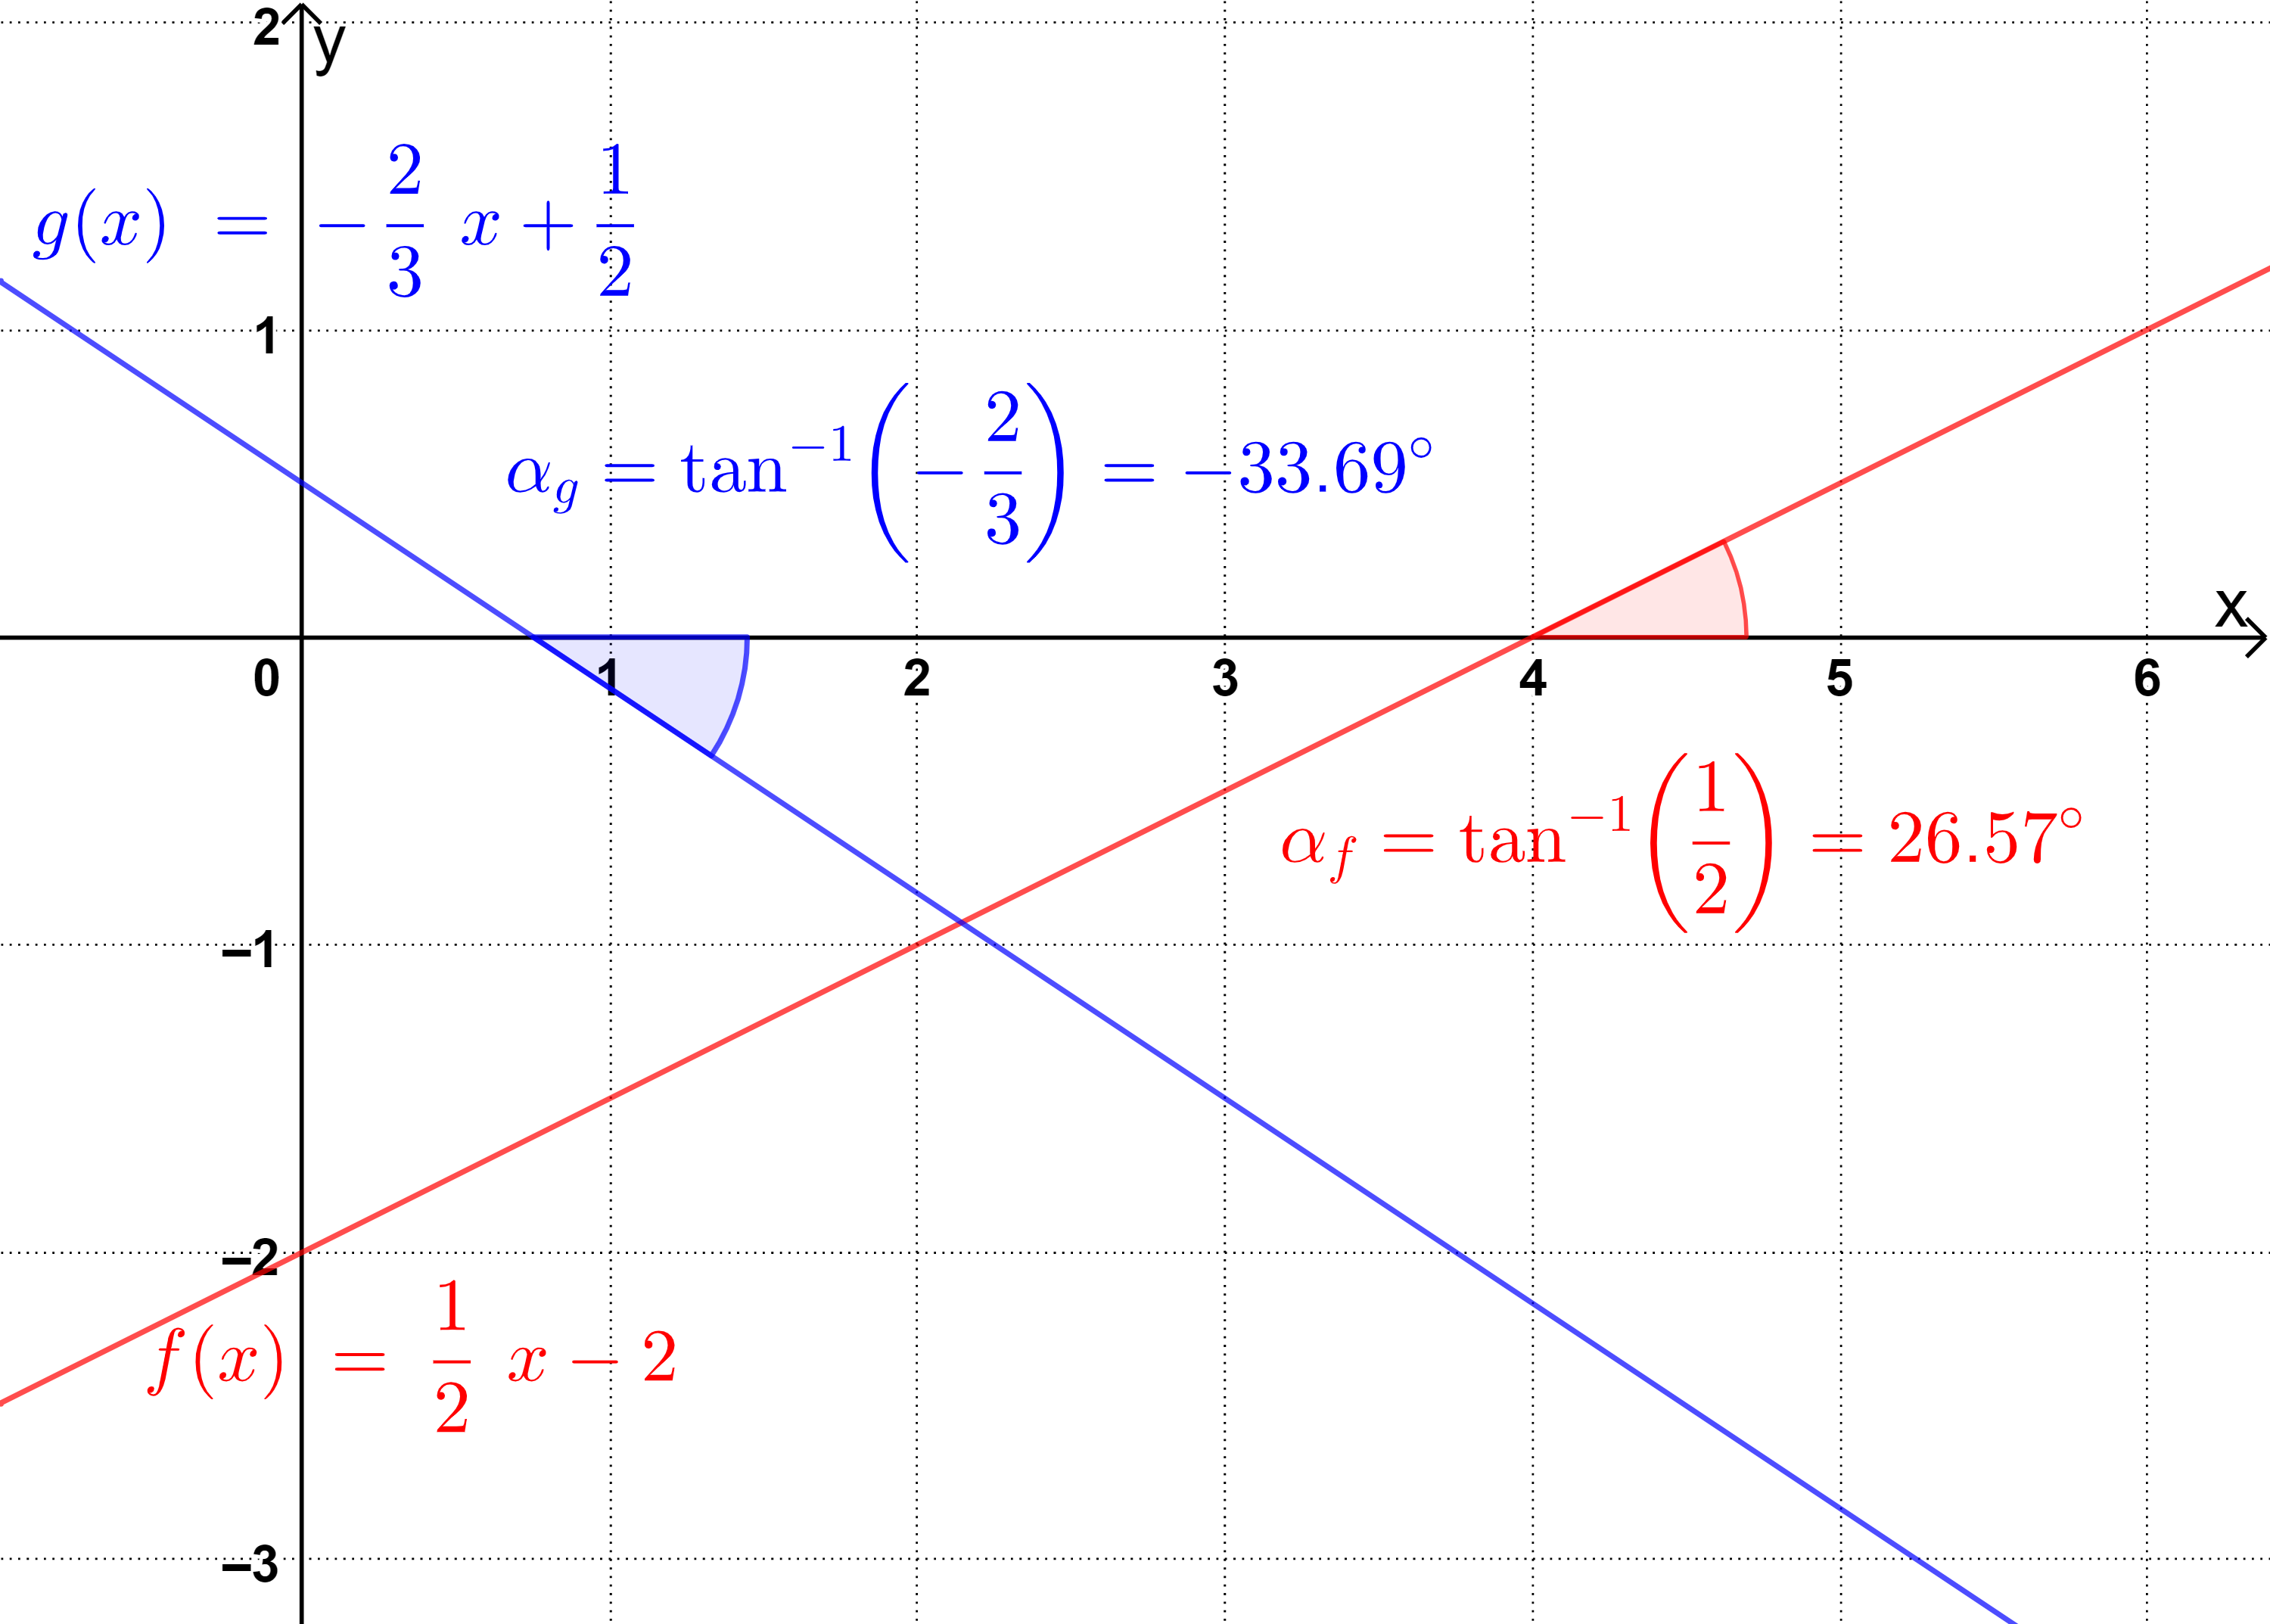
\includegraphics[width=0.8\textwidth]{\linFkt/pics/steigungswinkel.png}
\end{minipage}
Der Winkel zwischen der x-Achse und der Funktion wird als Steigungswinkel $\alpha$ bezeichnet. Man muss also immer an der x-Achse mit dem Messen des Winkels beginnen. Misst man den Winkel gegen den Uhrzeigersinn, so ist der Winkel positiv (siehe $\textcolor{red}{f(x)}$ im Beispiel), misst man im Uhrzeigersinn, so ist der Winkel positiv (siehe $\textcolor{blue}{g(x)}$ im Beispiel). Zwischen der Steigung $m$ und dem Steigungswinkel $\alpha$ gibt es folgenden Zusammenhang:\\
\begin{tcolorbox}
	\centering
	$\textcolor{loestc}{m=\tan\left(\alpha\right)\text{ und }\alpha=\tan^{-1}\left(m\right)}$
\end{tcolorbox}
\textbf{ACHTUNG:} Der Taschenrechner muss auf Gradmaß (degree bzw. deg) eingestellt sein.
\begin{Exercise}[title={Zeichne das Schaubild, miss den Steigungswinkel und vergleiche den Wert mit dem rechnerisch exakten.}, label=steigungswinkelA1]\\
	$f(x)=x-2 \qquad g(x)=2,5x-3 \qquad h(x)=-\dfrac{3}{4}x+2 \qquad i(x)=-1,5x-1$
\end{Exercise}
\newpage
\begin{Answer}[ref=steigungswinkelA1]\\
	\begin{minipage}{0.5\textwidth}
		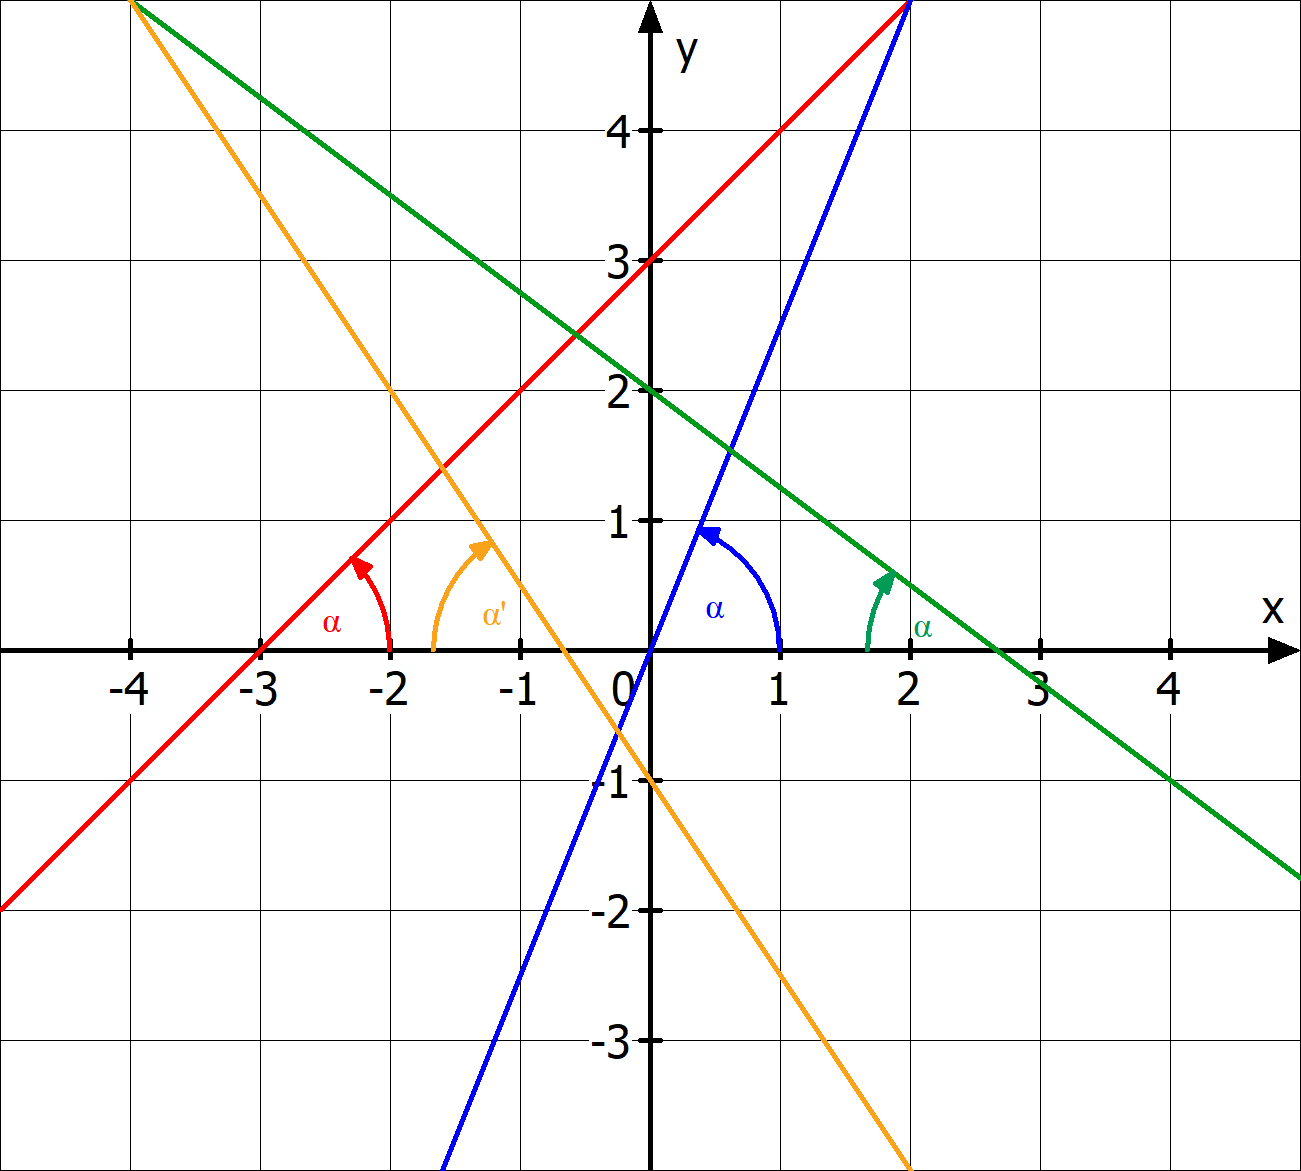
\includegraphics[width=0.95\textwidth]{\linFkt/pics/steigungswinkelA1_Loesung.png}
	\end{minipage}
	\begin{minipage}{0.5\textwidth}
		\begin{align*}
			\textcolor{red}{\alpha_f}&\textcolor{red}{=\tan^{-1}\left(1\right)=45^\circ}\\
			\textcolor{blue}{\alpha_g}&\textcolor{blue}{=\tan^{-1}\left(2,5\right)=68,20^\circ}\\
			\textcolor{ForestGreen}{\alpha_h}&\textcolor{ForestGreen}{=\tan^{-1}\left(-\dfrac{3}{4}\right)=-36,87^\circ}\\
			\textcolor{YellowOrange}{\alpha_i}&\textcolor{YellowOrange}{=\tan^{-1}\left(-1,5\right)=-56,31^\circ}
		\end{align*}
	\end{minipage}

\end{Answer}
